\cleardoublepage
\chapter{IMPLEMENTASI}
\label{chap:implementasi}

\section{Lingkungan Implementasi}

Konfigurasi lingkungan kerja (\textit{environment}) dilakukan untuk menjaga stabilitas eksekusi algoritma dan efisiensi pengolahan data. Tahap ini mencakup penyediaan infrastruktur perangkat keras serta instalasi dependensi perangkat lunak yang diperlukan dalam pemrosesan data deret waktu polusi udara. Pengaturan secara sistematis dilakukan agar model hibrida dapat melakukan komputasi matriks berdimensi tinggi secara stabil dan dapat direproduksi.

\subsection{Spesifikasi Perangkat Keras dan Perangkat Lunak}

Infrastruktur teknologi merupakan komponen dasar dalam eksekusi eksperimen sains data dalam penelitian ini. Lingkungan kerja dikonfigurasi untuk mendukung pengolahan data serta pelatihan model hibrida. Pengaturan perangkat keras dan perangkat lunak dilakukan dengan tujuan meminimalkan kendala teknis saat fase komputasi dan mengurangi nilai kesalahan estimasi model.

Spesifikasi perangkat keras yang digunakan mencakup kombinasi antara unit pemrosesan lokal dan berbasis awan (\textit{cloud}). Komputasi lokal menggunakan arsitektur sistem berbasis ARM pada perangkat MacBook Air M3 dengan kapasitas memori 16GB untuk tahap prapemrosesan awal dan penyusunan struktur kode program. 

Sementara itu, fase pelatihan model dan optimasi parameter menggunakan lingkungan awan berbasis \textit{Google Colab} versi gratis (\textit{Free Tier}). Penggunaan versi gratis ini dinilai sudah sangat memadai dan mencukupi untuk menangani seluruh rangkaian eksekusi kerangka kerja hibrida tanpa memerlukan alokasi peladen berbayar (\textit{Pro}). Secara eksplisit, spesifikasi \textit{hardware} standar yang disediakan oleh Google Colab gratis mencakup \textit{Central Processing Unit} (CPU) Intel(R) Xeon(R) @ 2.20GHz (2 vCPU) dengan alokasi \textit{System RAM} sebesar $\pm$12,7 GB, serta dukungan akselerasi \textit{Graphics Processing Unit} (GPU) NVIDIA T4 Tensor Core dengan \textit{Video RAM} (VRAM) sebesar 15 GB. 

Argumentasi ini sekaligus membuktikan efisiensi komputasional dari arsitektur hibrida sekuensial yang diusulkan. Karena proses pemisahan komponen non-linier (\textit{Random Forest}) dan linier (ARIMA) dipisahkan secara teratur, pemodelan ini tidak membutuhkan ruang memori masif tingkat tinggi (\textit{High-RAM}) ataupun waktu konvergensi yang eksponensial. Sistem operasi yang digunakan terdiri dari macOS Sequoia pada lingkungan lokal dan Ubuntu 22.04.3 LTS pada lingkungan awan. Bahasa pemrograman Python versi 3.10 ke atas dipilih sebagai bahasa utama karena ekosistem pustaka sains datanya menyediakan berbagai modul standardisasi analisis data yang terintegrasi. Rincian mengenai spesifikasi teknis dari perangkat keras dan perangkat lunak yang digunakan dalam penelitian ini disajikan secara sistematis pada Tabel \ref{tbl:spesifikasi_perangkat}.

\begin{table}[htbp]
\centering
\captionsetup{justification=centering}
\setlength{\tabcolsep}{6pt} 
\caption{Spesifikasi Lingkungan Implementasi Perangkat Keras dan Lunak}
\label{tbl:spesifikasi_perangkat}

\begin{tabularx}{\textwidth}{|>{\centering\arraybackslash}p{1.0cm}|
                              >{\raggedright\arraybackslash}p{3.5cm}|
                              >{\raggedright\arraybackslash}X|}
\hline
\textbf{No.} & \textbf{Komponen} & \textbf{Spesifikasi / Versi} \\
\hline
1 & Komputasi Lokal & Apple MacBook Air M3, RAM 16GB \\
\hline
2 & Komputasi \textit{Cloud} & Google Colab (Free Tier - Standard Runtime, T4 GPU, RAM 12.7GB) \\
\hline
3 & Sistem Operasi & macOS Sequoia (Lokal) / Ubuntu 22.04.3 LTS (\textit{Cloud}) \\
\hline
4 & Bahasa Pemrograman & Python 3.10+ \\
\hline
5 & \textit{Library} Utama & \texttt{pandas}, \texttt{scikit-learn}, \texttt{statsmodels}, \texttt{optuna}, \texttt{shap} \\
\hline
\end{tabularx}
\end{table}

\subsection{Inisialisasi Pustaka (\textit{Library Initialization})}

Tahapan pembuka dalam implementasi kode program melibatkan pemanggilan seluruh pustaka sains data yang diperlukan. Proses inisialisasi ini dilakukan untuk memuat berbagai modul yang menyediakan fungsi manipulasi struktur data serta algoritma pembelajaran mesin. Penyiapan pustaka dilakukan pada blok kode pertama untuk memastikan seluruh dependensi berada pada versi yang kompatibel dan dapat digunakan dalam setiap fungsi inferensi di dalam sistem, sebagaimana ditunjukkan pada Gambar \ref{gambar:inisialisasi_pustaka}.

Pustaka dasar seperti \texttt{pandas} dan \texttt{numpy} dimuat untuk keperluan manajemen data tabular dan operasi matriks numerik. Modul \texttt{statsmodels} diintegrasikan untuk memproses analisis deret waktu, termasuk dekomposisi musiman dan eksekusi model ARIMA pada komponen linier. Selain itu, modul \texttt{scikit-learn} digunakan sebagai instrumen dalam pembangunan komponen regresi non-linier berbasis \textit{Random Forest Regressor} (Regresi) serta penyediaan metrik evaluasi model.

Bagian akhir dari inisialisasi pustaka mencakup pemanggilan instrumen untuk pencarian parameter dan interpretasi model prediktif. Pustaka \texttt{optuna} diinisialisasi untuk menjalankan proses pencarian parameter berbasis probabilitas guna menemukan konfigurasi \textit{hyperparameter} yang sesuai bagi model hibrida secara otomatis. Terakhir, pustaka \texttt{shap} (\textit{SHapley Additive exPlanations}) dimuat untuk melakukan analisis \textit{Explainable AI} (XAI) yang bertujuan menguraikan kontribusi fitur terhadap hasil prediksi polusi harian Jakarta.

\begin{figure}[htbp]
  \centering
  \captionsetup{justification=centering}
  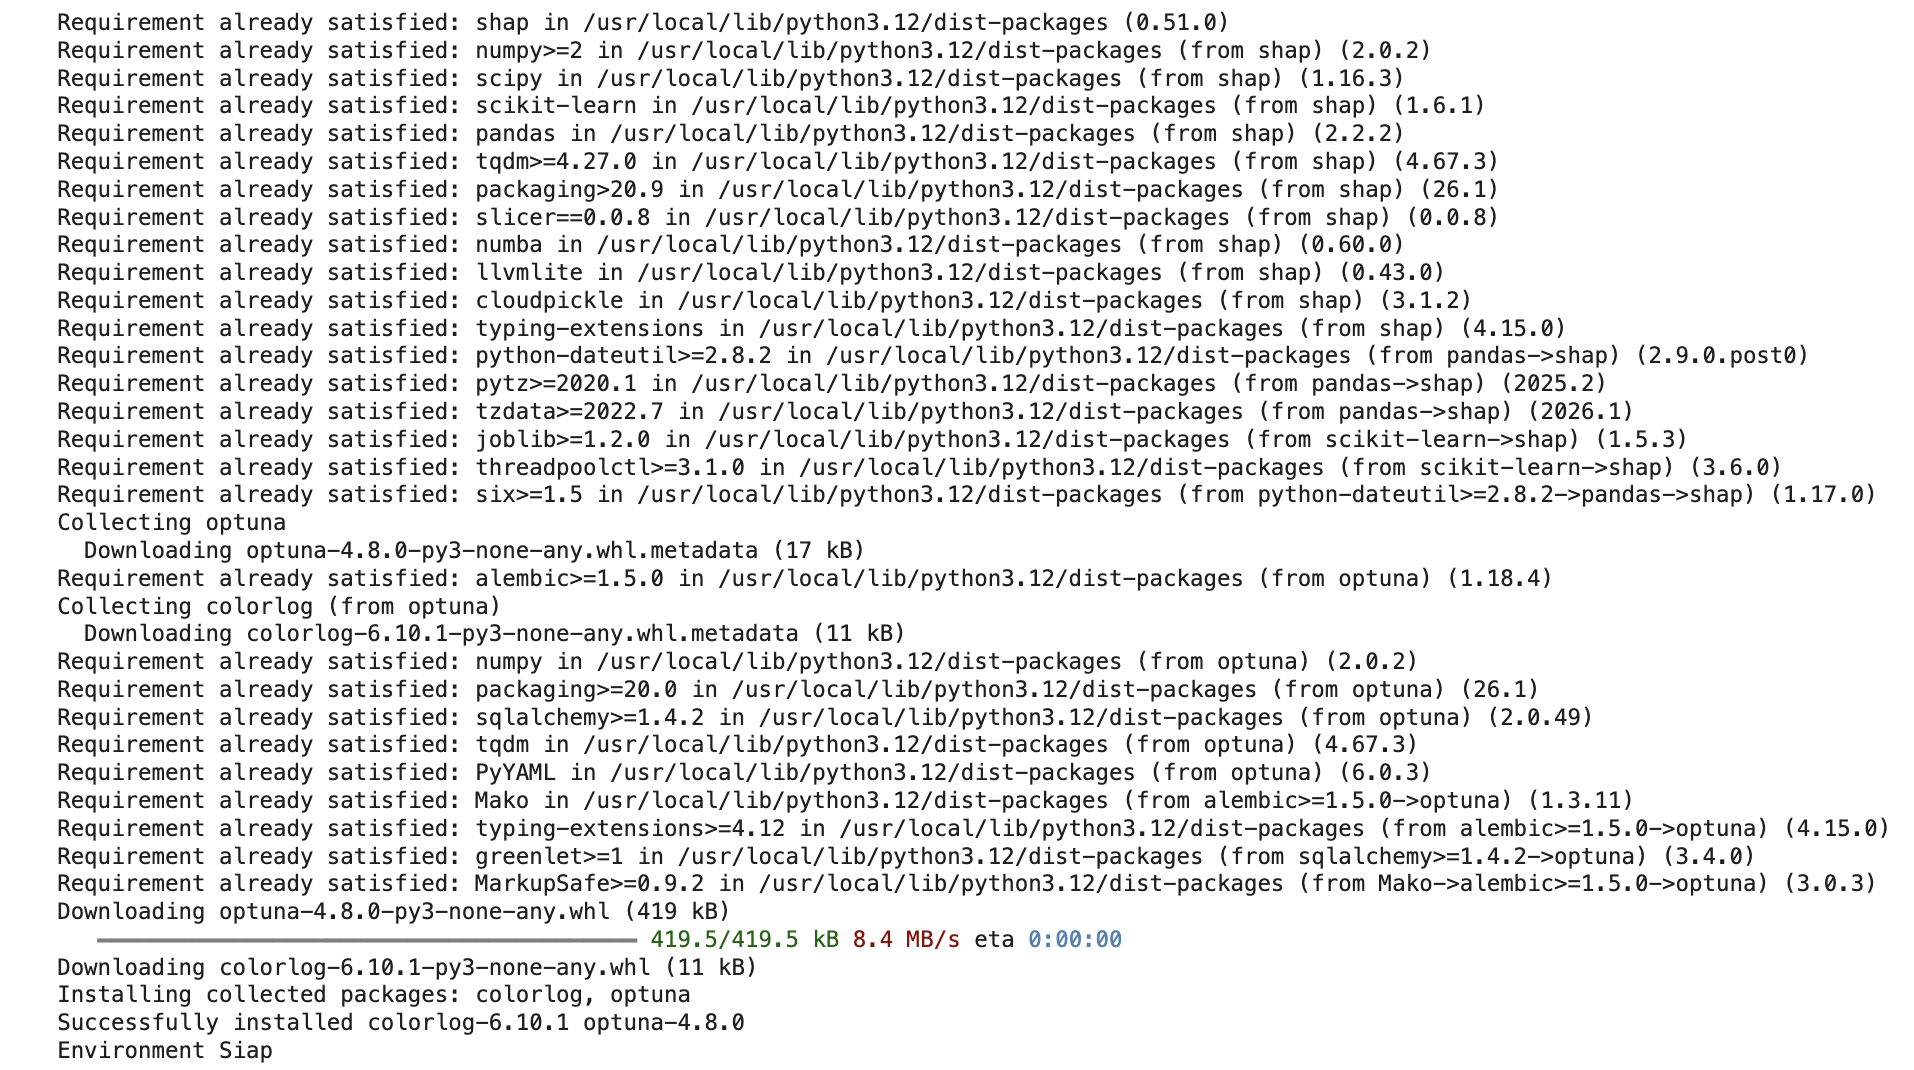
\includegraphics[width=0.6\textwidth]{images/0.png}
  \caption{Inisialisasi Lingkungan dan Pemanggilan Pustaka (\textit{Library})}
  \label{gambar:inisialisasi_pustaka}
\end{figure}

\section{Akuisisi dan Eksplorasi Data Awal (EDA)}

Data mentah kualitas udara dari Stasiun Pemantauan Kualitas Udara (SPKUA) Jakarta memuat rekaman historis konsentrasi polutan dari tahun 2010 hingga 2025. Tahapan ini menjabarkan proses integrasi data ke dalam sistem, mulai dari pemuatan awal hingga eksplorasi karakteristik statistik untuk menganalisis kelayakan data sebelum masuk ke fase pemodelan prediktif.

\subsection{Pemuatan dan Imputasi Deret Waktu}

Proses akuisisi data dilakukan dengan menarik berkas dataset dari repositori Google Drive. Pendekatan ini diterapkan agar alur pemrosesan data bersifat dinamis dan terpusat. Melalui metode ini, setiap perubahan pada berkas dataset di lingkungan \textit{cloud} dapat diproses pada tahapan inferensi tanpa memerlukan modifikasi ulang pada struktur kode program, sebagaimana implementasi penarikan data yang diilustrasikan pada Gambar \ref{gambar:load_data}.

\begin{figure}[htbp]
  \centering
  \captionsetup{justification=centering}
  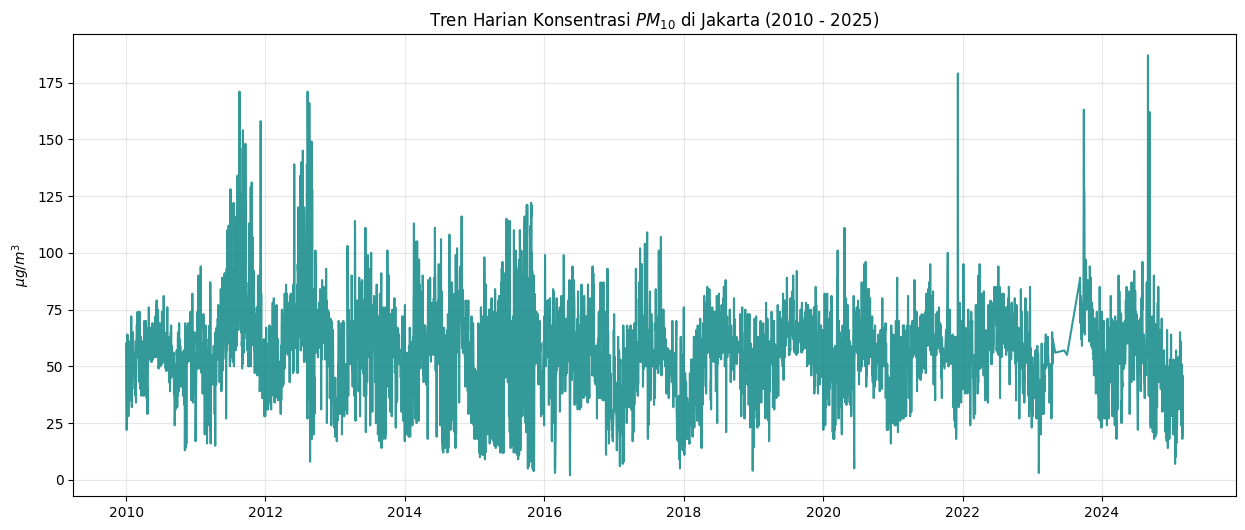
\includegraphics[width=0.6\textwidth]{images/1.png}
  \caption{Logika Pemuatan Data dan Interpolasi Deret Waktu}
  \label{gambar:load_data}
\end{figure}

Setelah data berhasil dimuat ke dalam lingkungan kerja, tahap selanjutnya adalah penyeragaman tipe matriks data. Setiap kolom yang merepresentasikan parameter polutan dikonversi ke dalam tipe numerik untuk memastikan kompatibilitas dengan fungsi matematika pada pustaka sains data. Sistem juga mengeksekusi perintah \texttt{df\_jakarta.reindex(all\_days)} untuk membangun indeks waktu yang utuh dan mengidentifikasi keberadaan tanggal yang tidak terekam dalam dataset asli.

\newpage

Keberadaan celah waktu (\textit{time gaps}) pada data dapat memengaruhi akurasi estimasi model deret waktu. Oleh karena itu, guna menghindari risiko kebocoran data (\textit{look-ahead bias}) pada fase pelatihan, baris data yang kosong pada set pelatihan diimputasi menggunakan metode rata-rata bergerak historis (\textit{historical rolling mean}) dengan jendela waktu mundur $k=5$. Sementara itu, pengisian mundur (\texttt{bfill()}) atau interpolasi berbasis waktu dapat diterapkan secara terbatas pada analisis tren makro non-pelatihan untuk menjaga kontinuitas visualisasi tanpa memengaruhi bobot inferensi kausal dari model hibrida.

\subsection{Analisis Data Hilang (\textit{Missing Values})}

Evaluasi terhadap persentase kekosongan data (\textit{missing values}) merupakan langkah untuk mengukur karakteristik pencatatan sensor sebelum observasi diproses lebih lanjut. Analisis ini menjadi dasar dalam menentukan strategi penanganan data yang sesuai agar tidak merubah distribusi pola asli data. Hasil identifikasi persentase kekosongan data untuk setiap parameter polutan disajikan secara visual pada Gambar \ref{gambar:missing_values}.

\begin{figure}[htbp]
  \centering
  \captionsetup{justification=centering}
  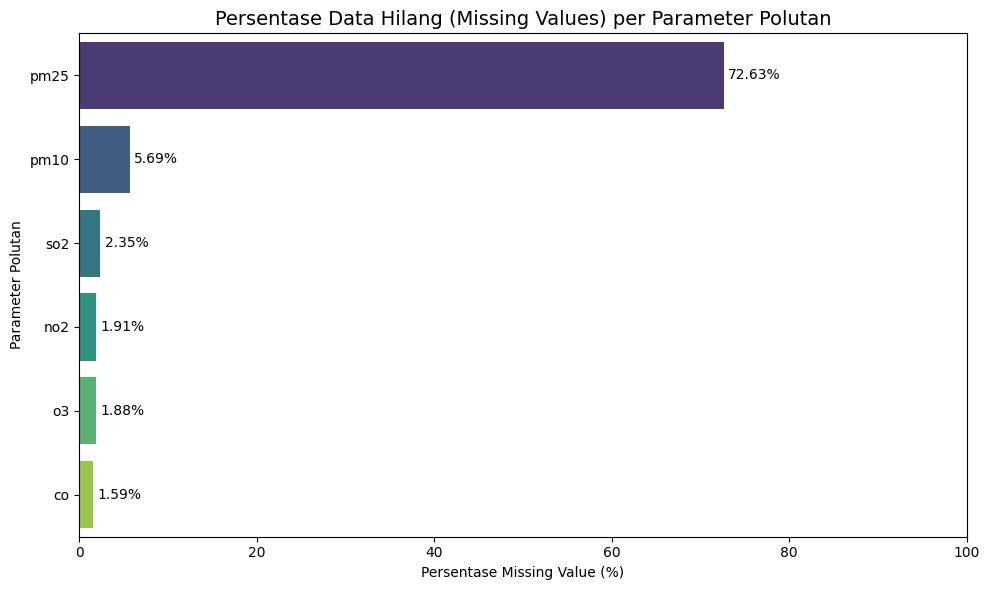
\includegraphics[width=0.6\textwidth]{images/4.png}
  \caption{Persentase \textit{Missing Values} pada Parameter Polutan}
  \label{gambar:missing_values}
\end{figure}

Berdasarkan hasil visualisasi tersebut, parameter $PM_{10}$ tercatat memiliki persentase data hilang tertentu dibandingkan dengan polutan gas lainnya. Fenomena kekosongan data ini merupakan karakteristik yang umum dijumpai pada sistem pemantauan lingkungan. Kondisi tersebut dapat dipengaruhi oleh faktor teknis perangkat sensor SPKUA di lapangan, kendala transmisi jaringan, atau adanya periode pemeliharaan kalibrasi rutin pada alat pantau.

Penerapan imputasi linear berbasis waktu mundur atau rata-rata bergerak historis dinilai sebagai pendekatan yang sesuai untuk karakteristik data deret waktu kualitas udara. Hal ini didasarkan pada sifat data kualitas udara yang kontinu dan memiliki keterikatan temporal, di mana nilai konsentrasi polutan umumnya tidak berubah secara ekstrem dalam interval waktu pendek. Proses imputasi historis ini menjaga kontinuitas deret waktu tanpa melanggar prinsip kronologis, sehingga pola musiman tetap konsisten saat diproses oleh komponen model hibrida sekuensial tanpa memicu bias informasi masa depan.

\subsection{Distribusi dan Keterkaitan Antarpolutan}

Analisis eksplorasi ini diimplementasikan untuk mengukur karakteristik spasial polusi antar wilayah di DKI Jakarta sekaligus mengevaluasi hubungan matematis antar variabel independen. Sistem menampilkan persebaran data parameter target $PM_{10}$ menggunakan \textit{Boxplot} dan kurva kepadatan, serta mengekstraksi Matriks Korelasi Pearson untuk mengidentifikasi potensi multikolinearitas dari polutan gas penyerta ($CO$, $NO_2$, $SO_2$, dan $O_3$). Hasil pemetaan sebaran konsentrasi partikulat dan matriks korelasi tersebut secara berturut-turut ditampilkan pada Gambar \ref{gambar:distribusi_stasiun} and Gambar \ref{gambar:korelasi_pearson}.

Berdasarkan visualisasi distribusi spasial di atas, dapat diamati tingkat kemiringan (\textit{skewness}) konsentrasi partikulat dan keberadaan nilai pencilan (\textit{outliers}) di masing-masing stasiun pemantau. Perbedaan distribusi ini menunjukkan bahwa setiap wilayah memiliki karakteristik emisi lokal yang bervariasi, sehingga evaluasi model prediktif dilakukan pada tingkat stasiun secara terpisah.

Pemahaman terhadap metrik korelasi antargas kemudian menjadi acuan empiris untuk proses rekayasa fitur pada tahap selanjutnya. Keberadaan korelasi antara polutan gas tertentu dengan $PM_{10}$ memberikan landasan teoretis untuk menyusun fitur interaksi kimiawi. Pemetaan ini dilakukan agar model \textit{Random Forest} Regresi menerima dimensi masukan yang secara karakteristik fisik dan kimiawi berkaitan dengan proses pembentukan polutan di udara.

\newpage

\begin{figure}[htbp]
  \centering
  \captionsetup{justification=centering}
  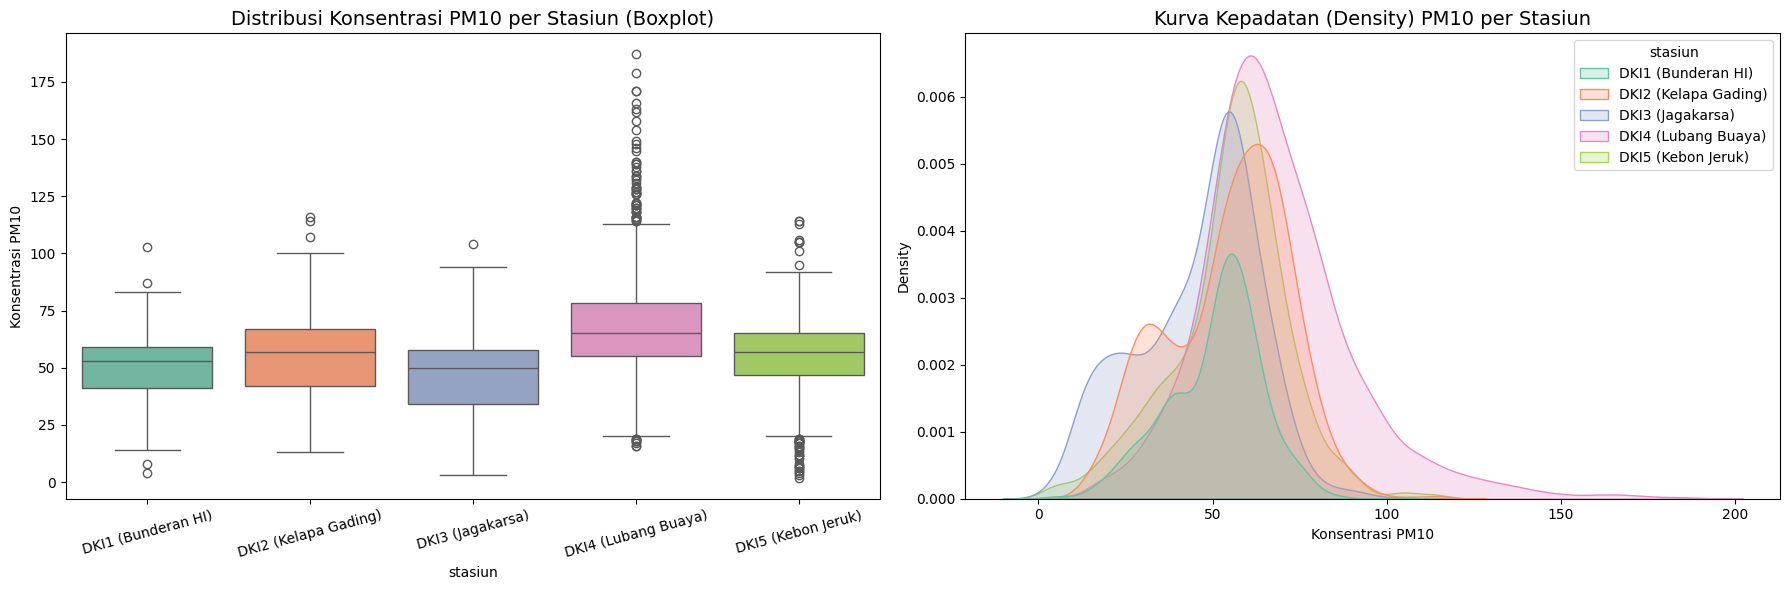
\includegraphics[width=0.6\textwidth]{images/2.png}
  \caption{Distribusi Konsentrasi PM\textsubscript{10} per Stasiun Pemantau}
  \label{gambar:distribusi_stasiun}
\end{figure}

\begin{figure}[htbp]
  \centering
  \captionsetup{justification=centering}
  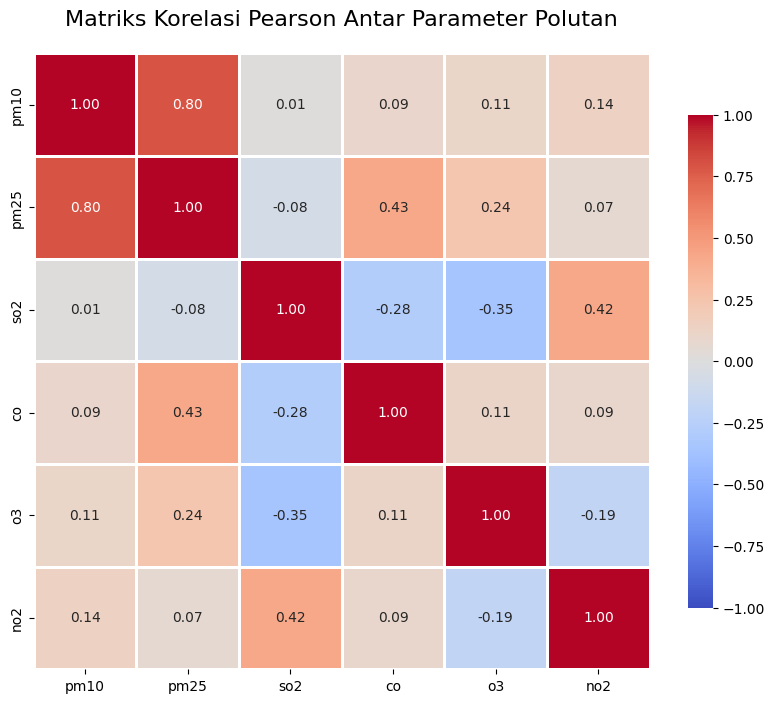
\includegraphics[width=0.6\textwidth]{images/3.png}
  \caption{Matriks Korelasi Pearson Antar Parameter Polutan}
  \label{gambar:korelasi_pearson}
\end{figure}

\subsection{Plot Tren Historis Stasiun (2010--2025)}

Validasi pergerakan data dalam jangka waktu panjang diperlukan untuk mengidentifikasi keberadaan siklus musiman dan variasi tren secara makro. Untuk memfasilitasi pengujian ini, kode program memuat fungsi perulangan (\textit{looping}) otomatis guna mengekstrak nilai metrik dan membangun visualisasi tren harian. Cuplikan implementasi kode program pencetakan grafik historis untuk setiap stasiun secara terpisah ditampilkan pada Gambar \ref{gambar:historis_kode}.

\begin{figure}[htbp]
  \centering
  \captionsetup{justification=centering}
  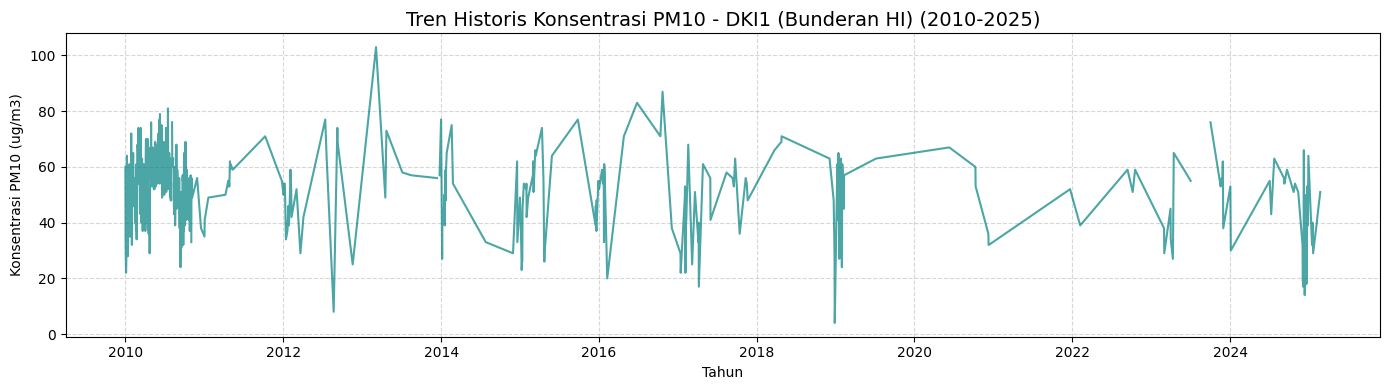
\includegraphics[width=0.6\textwidth]{images/5.png}
  \caption{Implementasi \textit{Looping} Visualisasi Historis dan Ekstraksi Statistik}
  \label{gambar:historis_kode}
\end{figure}

Melalui hasil perulangan pencetakan visualisasi tersebut, teridentifikasi adanya pola musiman tahunan pada seluruh stasiun pemantauan. Konsentrasi $PM_{10}$ memiliki tendensi kenaikan pada rentang waktu pertengahan tahun, yang secara klimatologis bertepatan dengan siklus musim kemarau. Visualisasi observasi juga menunjukkan adanya penurunan polutan pada periode 2020 hingga 2021, yang bertepatan dengan kebijakan pembatasan mobilitas fisik saat pandemi COVID-19.

Kehadiran fluktuasi musiman yang siklikal serta variasi tren dari faktor eksternal menunjukkan bahwa data deret waktu kualitas udara ini bersifat non-stasioner. Temuan empiris dari tahap rekayasa data awal ini menjadi dasar pertimbangan mengapa pendekatan regresi linear tunggal memiliki batasan dalam memproses varians data. Hal ini menunjukkan perlunya penerapan komponen deret waktu khusus, seperti algoritma persamaan diferensi stokastik ARIMA, untuk memodelkan variansi temporal dengan tingkat galat yang minimum.

\section{Analisis Stasioneritas dan Dekomposisi Musiman}

Syarat sebelum membangun pemodelan menggunakan komponen linier seperti ARIMA adalah memastikan bahwa data deret waktu memenuhi kriteria stasioneritas. Tahapan implementasi pada bagian ini mencakup evaluasi keterikatan temporal, pemisahan komponen musiman melalui analisis dekomposisi, serta pengujian stasioneritas secara statistik. Rangkaian analisis ini dilakukan untuk mengidentifikasi karakteristik intrinsik data sebelum diproses ke dalam arsitektur hibrida.

\subsection{Korelasi Silang (Cross-Correlation Function / CCF)}

Pencarian nilai jeda waktu (\textit{lag}) yang sesuai dilakukan dengan mengukur tingkat korelasi antara variabel eksogen terhadap target $PM_{10}$ menggunakan Fungsi Korelasi Silang (CCF). Evaluasi ini bertujuan untuk menganalisis pengaruh karakteristik nilai historis polutan gas pada periode sebelumnya terhadap pembentukan partikulat pada waktu target. Pemetaan nilai korelasi pada interval waktu mundur tersebut diimplementasikan melalui kode program yang ditunjukkan pada Gambar \ref{gambar:ccf}.

\begin{figure}[htbp]
  \centering
  \captionsetup{justification=centering}
  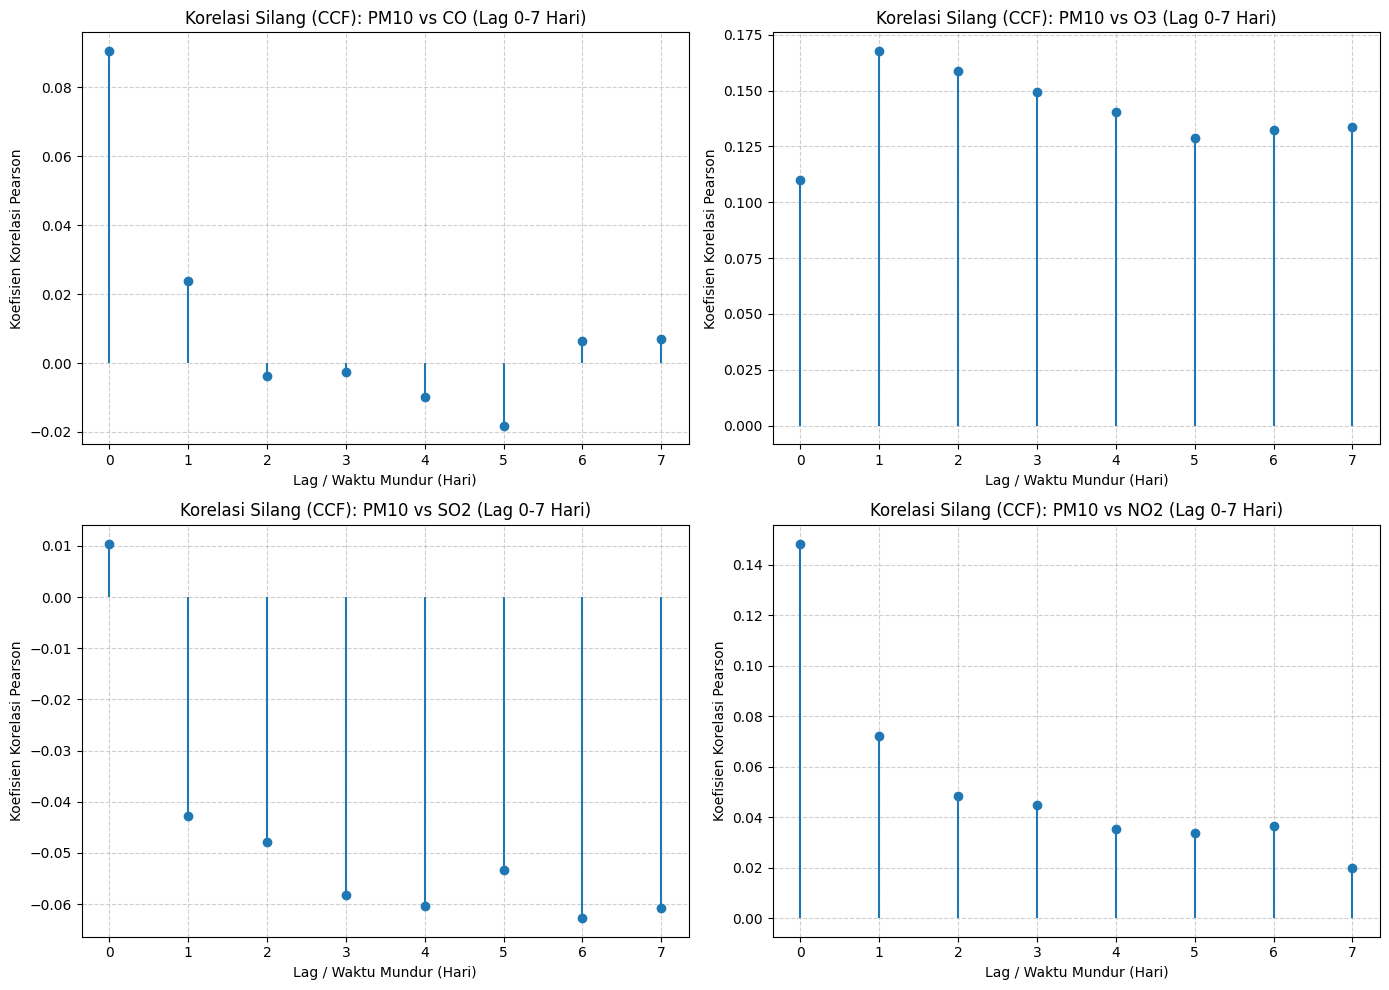
\includegraphics[width=0.6\textwidth]{images/11.png}
  \caption{Implementasi Plot Fungsi Korelasi Silang (CCF) dengan Lag 0-7 Hari}
  \label{gambar:ccf}
\end{figure}

Kode komputasi CCF tersebut melakukan kalkulasi pada berbagai parameter gas penyerta untuk menghitung koefisien korelasi silang pada rentang waktu nol hingga tujuh hari ke belakang. Penggunaan rentang observasi selama satu minggu dinilai memadai untuk memetakan karakteristik siklus akumulasi polutan harian di atmosfer perkotaan tanpa membebani model dengan fitur masa lalu yang nilai korelasinya telah menurun. Nilai yang mendekati batas statistik kemudian diekstrak sebagai kandidat atribut prediktor.

Hasil dari pemetaan korelasi ini menunjukkan bahwa beberapa polutan gas penyerta memiliki efek tunda (\textit{delayed effect}) terhadap konsentrasi partikulat utama. Informasi ini digunakan untuk memandu proses rekayasa fitur pada tahap selanjutnya, di mana variabel dengan korelasi pada \textit{lag} tertentu ditransformasikan menjadi atribut baru. Langkah tersebut ditujukan agar model pembelajaran mesin menerima dimensi masukan yang memiliki kapabilitas estimasi berdasarkan data historis.

\subsection{Dekomposisi Deret Waktu Aditif}

Data karakteristik kualitas udara mengandung berbagai pola yang bervariasi, sehingga dipisahkan menggunakan metode dekomposisi deret waktu aditif. Proses ekstraksi ini memecah data historis ke dalam tiga dimensi, yaitu komponen tren, komponen musiman (\textit{seasonal}), dan komponen residu (\textit{noise}). Operasi pemisahan matematis ini dieksekusi menggunakan fungsi \texttt{seasonal\_decompose} dari pustaka sains data yang diilustrasikan pada Gambar \ref{gambar:dekomposisi}.

\begin{figure}[htbp]
  \centering
  \captionsetup{justification=centering}
  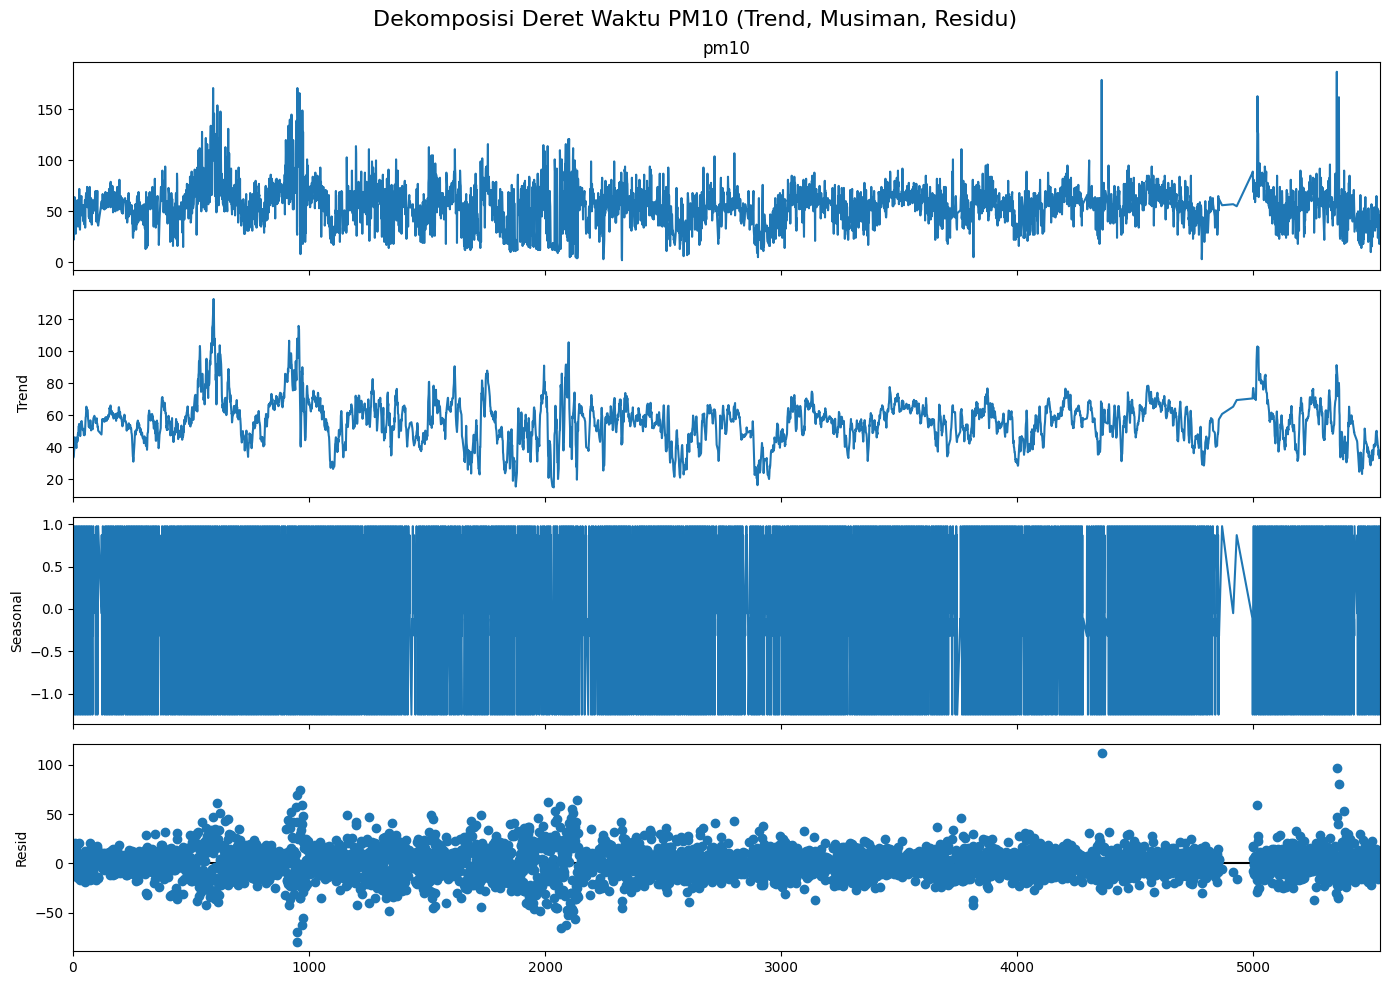
\includegraphics[width=0.6\textwidth]{images/12.png}
  \caption{Komputasi dan Visualisasi Dekomposisi Aditif Deret Waktu PM\textsubscript{10}}
  \label{gambar:dekomposisi}
\end{figure}

Komponen tren pada hasil dekomposisi merepresentasikan arah pergerakan konsentrasi polutan dalam jangka waktu panjang, yang tidak dipengaruhi oleh fluktuasi harian. Di sisi lain, komponen musiman memetakan pola periodik yang berulang secara teratur pada rentang waktu tertentu setiap tahunnya. Sementara itu, komponen residu menyajikan variansi sisa yang tidak dijelaskan oleh tren maupun pola musiman, yang merepresentasikan kejadian anomali atmosferik atau efek acak.

Pemisahan ketiga dimensi analitik ini memberikan gambaran mengenai stabilitas ragam (\textit{variance}) dan rata-rata (\textit{mean}) data dari waktu ke waktu. Visualisasi hasil dekomposisi mempermudah evaluasi stasioneritas secara visual sebelum pergerakan data divalidasi dengan pengujian statistik. Penanganan terhadap fluktuasi musiman yang terdeteksi ini akan diselesaikan melalui algoritma penyesuaian parameter diferensi pada tahap pemodelan ARIMA.

\subsection{Uji Stasioneritas (ADF dan KPSS Test)}

Pengujian stasioneritas melalui analisis visual memiliki batasan, sehingga validasi kuantitatif menggunakan uji statistik formal diperlukan. Evaluasi kuantitatif ini dijalankan untuk memastikan sifat stasioneritas pada data runtun waktu kualitas udara sebelum memasuki tahapan pemodelan statistik konvensional. Penentuan kondisi stasioner ini menjadi parameter penting karena memengaruhi keandalan model dalam memproyeksikan komponen data linier.

Penerapan uji silang antara uji \textit{Augmented Dickey-Fuller} (ADF) dan \textit{Kwiatkowski-Phillips-Schmidt-Shin} (KPSS) dipilih untuk mengonfirmasi kondisi stasioneritas secara lebih terukur dan menghindari kesalahan interpretasi. Uji statistik ADF berfokus pada deteksi keberadaan akar unit (\textit{unit root}), di mana penolakan hipotesis nol mengindikasikan bahwa data tersebut stasioner. Sebaliknya, uji KPSS memiliki landasan hipotesis nol berupa konfirmasi bahwa data memiliki sifat stasioner, sehingga kombinasi keduanya menghasilkan simpulan yang lebih berimbang. Kerangka fungsi komputasi yang dirancang untuk menjalankan pengujian gabungan ini disajikan pada Gambar \ref{gambar:uji_adf}.

\begin{figure}[htbp]
  \centering
  \captionsetup{justification=centering}
  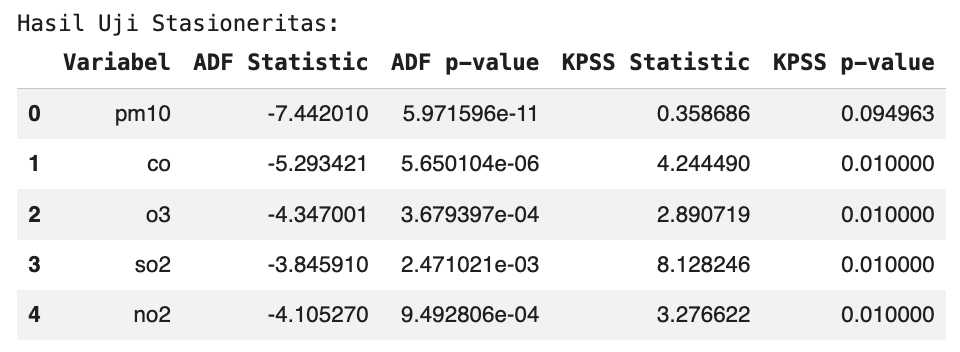
\includegraphics[width=0.6\textwidth]{images/13.png}
  \caption{Implementasi Skrip Evaluasi Stasioneritas Data}
  \label{gambar:uji_adf}
\end{figure}

Hasil penaksiran nilai signifikansi ($p$-value) yang dikembalikan oleh kedua pengujian tersebut menjadi acuan dasar dalam memandu penentuan parameter integrasi atau pembedaan (\textit{differencing}, $d$) yang dibutuhkan oleh komponen ARIMA. Apabila kedua pengujian menunjukkan karakteristik hasil yang bervariasi, data dikategorikan stasioner secara parsial, dan penyesuaian matematis lanjutan dapat dipertimbangkan sebelum komponen utama model hibrida sekuensial dilatih. Ringkasan hasil perhitungan angka statistik untuk seluruh parameter polutan udara tersebut dirangkum pada Tabel \ref{tbl:hasil_stasioneritas}.

\begin{table}[htbp]
\centering
\captionsetup{justification=centering}
\setlength{\tabcolsep}{4pt} 
\caption{Hasil Komputasi Uji Stasioneritas ADF dan KPSS}
\label{tbl:hasil_stasioneritas}

\begin{tabularx}{\textwidth}{|>{\raggedright\arraybackslash}X|
                              >{\centering\arraybackslash}p{2.3cm}|
                              >{\centering\arraybackslash}p{2.3cm}|
                              >{\centering\arraybackslash}p{2.3cm}|
                              >{\centering\arraybackslash}p{2.3cm}|}
\hline
\textbf{Variabel} & \textbf{ADF Statistic} & \textbf{ADF $p$-value} & \textbf{KPSS Stat} & \textbf{KPSS $p$-value} \\
\hline
$\text{PM}_{10}$ & -7,4420 & 0,0000 & 0,3587 & 0,0950 \\
\hline
$\text{CO}$ & -5,2934 & 0,0000 & 4,2445 & 0,0100 \\
\hline
$\text{O}_3$ & -4,3470 & 0,0004 & 2,8907 & 0,0100 \\
\hline
$\text{SO}_2$ & -3,8459 & 0,0025 & 8,1282 & 0,0100 \\
\hline
$\text{NO}_2$ & -4,1053 & 0,0009 & 3,2766 & 0,0100 \\
\hline
\end{tabularx}
\end{table}

\section{Implementasi Rekayasa Fitur (\textit{Feature Engineering})}

Bagian ini merealisasikan rancangan penambahan dimensi matriks berdasarkan karakteristik kimiawi polutan dan dependensi temporal. Proses rekayasa fitur dilakukan untuk mengekstraksi informasi temporal dan karakteristik kimiawi dari variabel mentah sehingga model hibrida dapat memproses hubungan non-linier yang memengaruhi konsentrasi $PM_{10}$ di atmosfer Jakarta.

\subsection{Pembangkitan Matriks Fitur Komposit}

Pembangkitan fitur komposit diimplementasikan dengan menambahkan atribut masukan yang relevan secara domain untuk memfasilitasi proses estimasi model. Proses ini melibatkan transformasi data deret waktu mentah menjadi variabel turunan yang merepresentasikan dinamika polutan dalam berbagai skala waktu. 

Transformasi temporal dilakukan dengan menerapkan operasi \textit{shifting} untuk menghasilkan fitur jeda temporal (\textit{lag}) yang menangkap dependensi jangka pendek dari kualitas udara pada hari-hari sebelumnya. Selain itu, digunakan operasi jendela berjalan (\textit{rolling window}) guna mengekstrak statistik bergerak seperti nilai rata-rata (\textit{mean}) 3-hari dan 7-hari, serta standar deviasi 7-hari. Pendekatan ini digunakan agar komponen \textit{Random Forest} Regresi dapat memproses tren fluktuasi polutan dan stabilitas variansi data secara terstruktur.

Sistem juga membentuk fitur interaksi khusus \texttt{co\_times\_o3} yang merepresentasikan karakteristik laju pembentukan polutan sekunder melalui mekanisme reaksi fotokimia di atmosfer. Atribut kategorikal tambahan seperti \texttt{season} (musim) dan \texttt{is\_weekend} (indikator akhir pekan) diintegrasikan untuk menangkap variasi aktivitas harian manusia serta kondisi meteorologi lokal. Integrasi fitur-fitur ini digunakan untuk menyediakan karakteristik domain sains atmosfer bagi model hibrida dalam memetakan hubungan non-linier antara polutan gas dan partikulat target.

\section{Skema Validasi dan Pemisahan Data}

Skema validasi digunakan untuk menguji kemampuan generalisasi model terhadap data yang tidak digunakan dalam proses pelatihan. Untuk meminimalkan risiko kebocoran informasi masa depan ke masa lalu (\textit{look-ahead bias}), pemisahan data dilakukan secara temporal berdasarkan urutan waktu. Pendekatan ini ditujukan untuk menjaga konsistensi evaluasi data deret waktu agar tetap sesuai dengan urutan kronologis data kualitas udara di lapangan.

\subsection{Pemisahan Set Pelatihan dan Pengujian}

Tahap awal evaluasi melibatkan pembagian dataset menjadi dua bagian utama, yaitu data pelatihan (\textit{training set}) dan data pengujian (\textit{testing set}) dengan proporsi masing-masing sebesar 80\% dan 20\%. Pembagian ini dilakukan secara kronologis berdasarkan urutan waktu guna menyimulasikan kondisi operasional nyata, di mana model dikondisikan untuk melakukan penaksiran nilai pada periode waktu setelah masa pelatihan selesai.

\begin{figure}[htbp]
  \centering
  \captionsetup{justification=centering}
  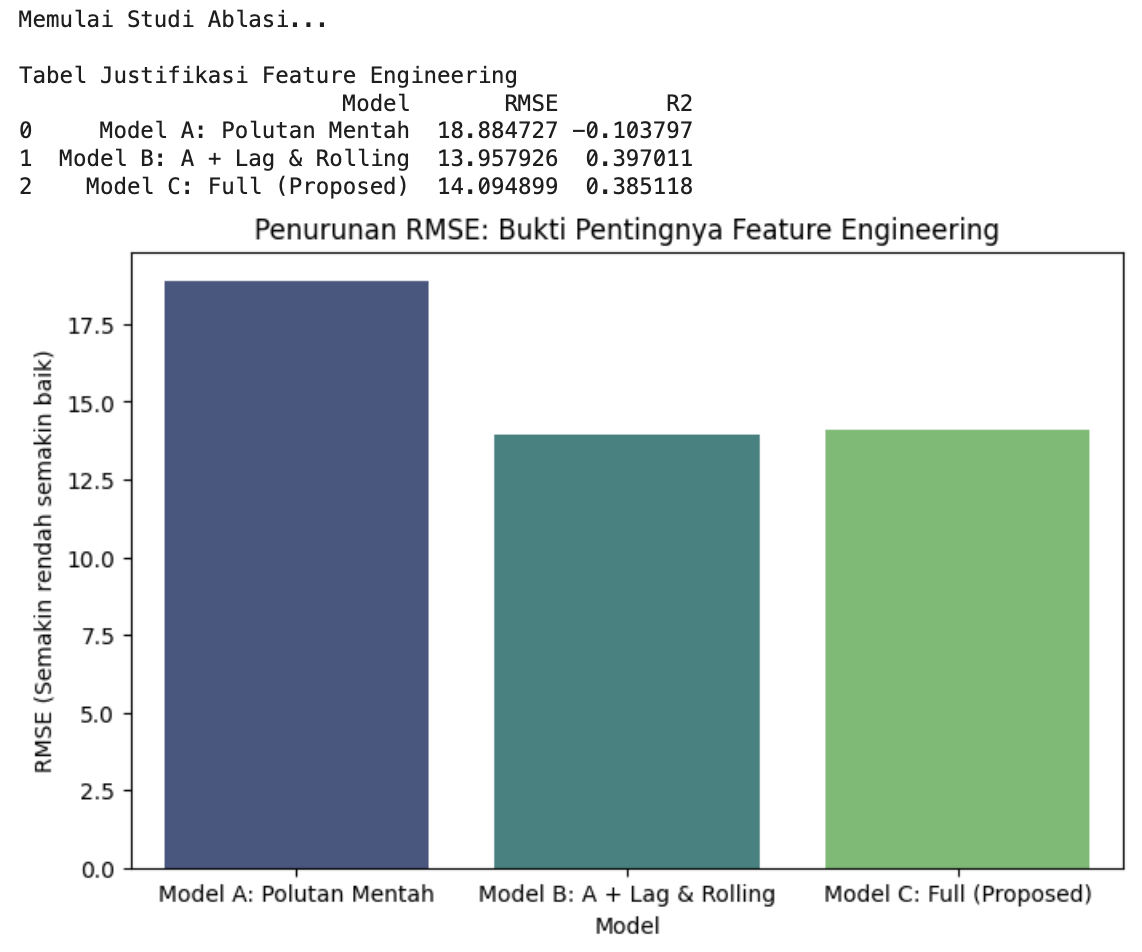
\includegraphics[width=0.6\textwidth]{images/15.png}
  \caption{Pemotongan Data Latih dan Uji secara Kronologis}
  \label{gambar:train_test_split}
\end{figure}

Berbeda dengan data tabular konvensional yang dapat diacak (\textit{shuffled}), data deret waktu kualitas udara memiliki dependensi temporal yang saling terikat antar-waktu. Proses pengacakan baris data dihindari karena berpotensi memicu kebocoran informasi dari periode masa depan ke dalam proses pelatihan masa lalu, yang dapat menghasilkan nilai kesalahan yang bias (\textit{overoptimistic results}). Oleh karena itu, pemotongan indeks data dilakukan secara berurutan mulai dari tanggal awal hingga batas waktu pemisahan guna memastikan data pengujian tetap terisolasi hingga fase evaluasi dilakukan, sebagaimana disajikan pada Gambar \ref{gambar:train_test_split}.

\subsection{Validasi Silang Deret Waktu (\textit{TimeSeriesSplit})}

Untuk menjaga stabilitas evaluasi selama fase pelatihan tanpa merusak kronologi alami data, digunakan metode validasi silang deret waktu dengan pendekatan \textit{Forward Chaining} berbasis 5-\textit{fold}. Berbeda dengan metode \textit{K-Fold} konvensional yang melakukan pengacakan data, pendekatan ini bekerja dengan memperluas jendela data latih secara bertahap sehingga subset data validasi selalu berada pada periode waktu setelah data pelatihan. Mekanisme ini diterapkan agar konfigurasi parameter model hibrida sekuensial dapat beradaptasi terhadap dependensi temporal polutan PM\textsubscript{10} di Jakarta guna menghasilkan estimasi nilai galat yang representatif terhadap variasi data runtun waktu. Prosedur operasional dari rangkaian eksperimen validasi silang ini dijabarkan pada Algoritma \ref{alg:time_series_split}, sedangkan implementasi penempatan skrip perulangannya pada tingkat kode program disajikan pada Gambar \ref{gambar:tscv_code}.

\begin{algorithm}[htbp]
\caption{Algoritma Validasi Silang \textit{TimeSeriesSplit} (5-Fold)}
\label{alg:time_series_split}
\begin{algorithmic}[1]
\Require Matriks fitur latih $X_{train}$, Vektor target latih $Y_{train}$
\Ensure Array rata-rata skor evaluasi $\overline{RMSE}$

\State $Scores \gets \emptyset$ \Comment{Inisialisasi himpunan skor kosong}
\State Inisialisasi pembagian berantai (\textit{Forward Chaining}) untuk $K=5$
\For{\textbf{each} $(X_{tr}, Y_{tr})$ dan $(X_{vl}, Y_{vl})$ \textbf{dalam} Partisi}
    \State $\hat{N}_{tr} \gets \text{Latih dan Prediksi } RandomForest(X_{tr}, Y_{tr})$
    \State $Residu \gets Y_{tr} - \hat{N}_{tr}$
    \State $\hat{L}_{vl} \gets \text{Latih dan Peramal } ARIMA(Residu, \text{langkah} = |Y_{vl}|)$
    
    \State $\hat{Y}_{hybrid} \gets RandomForest.predict(X_{vl}) + \hat{L}_{vl}$
    \State $Error \gets \sqrt{\frac{1}{|Y_{vl}|} \sum (Y_{vl} - \hat{Y}_{hybrid})^2}$
    \State $Scores \gets Scores \cup \{Error\}$ 
\EndFor

\State \Return $\text{Mean}(Scores)$
\end{algorithmic}
\end{algorithm}

\begin{figure}[htbp]
  \centering
  \captionsetup{justification=centering}
  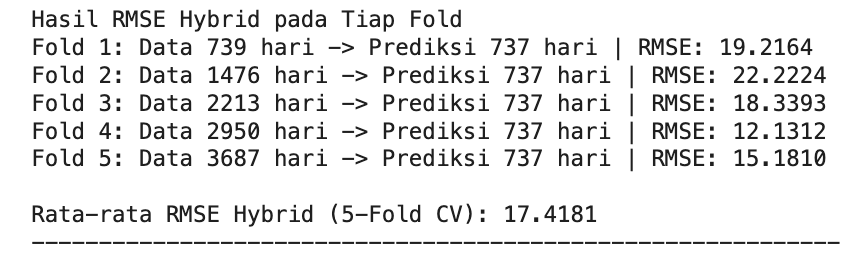
\includegraphics[width=0.8\textwidth]{images/16.png}
  \caption{Implementasi Perulangan 5-Fold TimeSeriesSplit}
  \label{gambar:tscv_code}
\end{figure}

\section{Implementasi Model Hibrida Sekuensial}

Tahapan ini menguraikan realisasi kode program untuk mengintegrasikan \textit{Random Forest} Regresi sebagai komponen pemodelan non-linier dengan ARIMA sebagai komponen pemodelan linier ke dalam satu alur (\textit{pipeline}) estimasi harian. Struktur hibrida sekuensial ini disusun untuk memanfaatkan karakteristik masing-masing algoritma dalam memproses komponen data yang bervariasi. Proses integrasi ini dilakukan agar residu atau galat yang tidak terpetakan oleh model primer dapat dikoreksi oleh model sekunder melalui pendekatan deret waktu.

\subsection{Fase Primer dan Penyetelan Parameter menggunakan Optuna}

Implementasi tahap primer berfokus pada pembangunan komponen non-linier menggunakan algoritma \textit{Random Forest Regressor} (Regresi). Pemilihan algoritma ini didasarkan pada karakteristiknya dalam memproses interaksi antarfitur secara multivariat dan parameter data yang bervariasi tanpa memerlukan asumsi distribusi normal. Fase ini digunakan untuk memodelkan pola utama dari fluktuasi konsentrasi polutan PM\textsubscript{10} berdasarkan fitur-fitur dasar dan rekayasa fitur yang telah dibentuk sebelumnya.

Penyetelan konfigurasi model primer dilakukan melalui pencarian \textit{hyperparameter} secara sistematis untuk meminimalkan risiko model mengalami kondisi penyesuaian berlebih (\textit{overfitting}). Proses pencarian parameter dieksekusi menggunakan pencarian probabilistik Bayesian melalui pustaka \texttt{optuna} yang mengevaluasi kombinasi parameter berdasarkan riwayat iterasi sebelumnya untuk mengefisiensikan waktu komputasi. Penyetelan ini secara spesifik mengevaluasi parameter seperti jumlah pohon (\texttt{n\_estimators}) serta kedalaman maksimum pohon (\texttt{max\_depth}) guna meminimalkan fungsi nilai kesalahan (\textit{validation RMSE}).

Konfigurasi parameter yang diperoleh dari fase pencarian tersebut kemudian disimpan sebagai model dasar dalam struktur hibrida sekuensial. Nilai prediksi primer yang dihasilkan oleh model ini diekstrak menjadi variabel masukan untuk tahap pemodelan residu linier di fase selanjutnya. 

\subsection{Ekstraksi Residu dan Pemodelan Fase Sekunder}

Setelah fase primer selesai, sistem melakukan kalkulasi ekstraksi nilai residu yang didefinisikan sebagai selisih matematis antara nilai observasi aktual dengan hasil prediksi \textit{Random Forest} Regresi. Data residu ini dianalisis karena mengandung komponen informasi temporal linier yang tidak dipetakan oleh model berbasis pohon akibat karakteristik algoritmanya yang tidak mempertimbangkan dependensi temporal secara intrinsik. Eksplorasi terhadap sifat autokorelasi data sisaan galat ini dilakukan melalui analisis plot ACF dan PACF untuk menentukan orde ARIMA yang sesuai, sebagaimana diilustrasikan pada Gambar \ref{gambar:arima_res}.

Komponen linier ARIMA selanjutnya dilatih menggunakan deret waktu residu tersebut untuk menangkap dependensi temporal yang masih tertinggal dalam data sisaan. Integrasi antara model primer dan sekunder dilakukan secara sekuensial, di mana luaran dari fase pertama menjadi masukan bagi fase kedua. Proses pelatihan ini bertujuan untuk meminimalkan autokorelasi pada galat estimasi sehingga komponen ARIMA dapat mendeteksi tren linier lokal, di mana logika operasional dari keseluruhan alur pelatihan dan inferensi sekuensial ini dirangkum secara sistematis pada Algoritma \ref{alg:hybrid_training_final}.

\begin{figure}[htbp]
  \centering
  \captionsetup{justification=centering}
  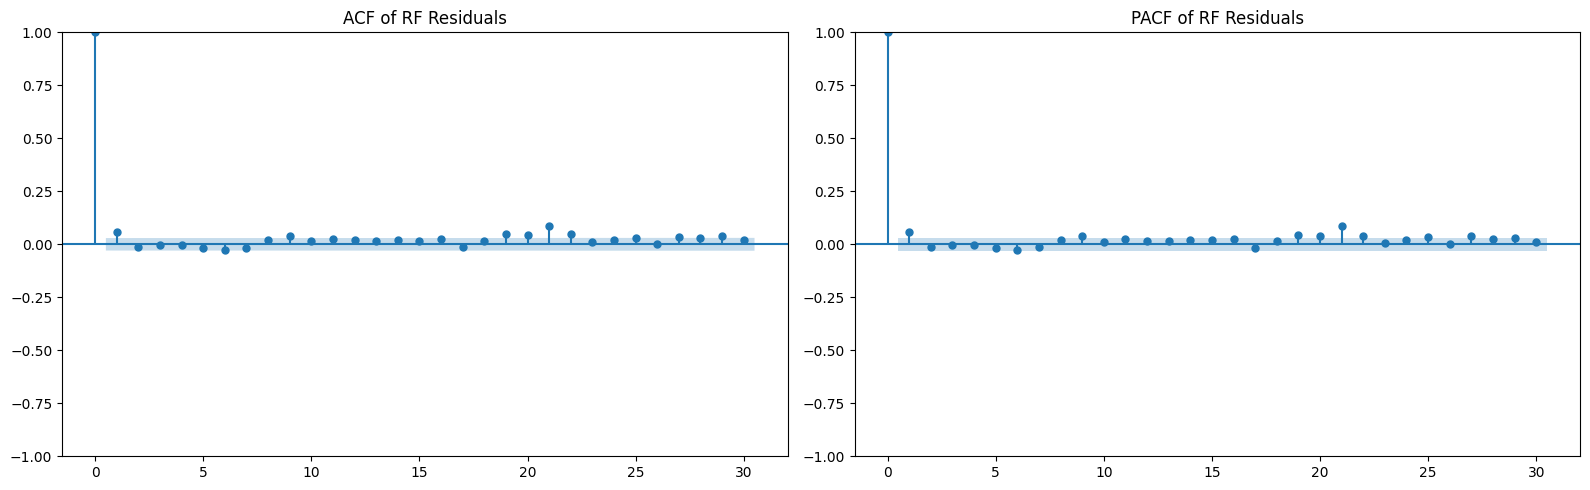
\includegraphics[width=0.8\textwidth]{images/18.png}
  \caption{Plot ACF/PACF Residu dan Pelatihan Model ARIMA Sekunder}
  \label{gambar:arima_res}
\end{figure}

\begin{algorithm}[htbp]
\caption{Pelatihan dan Inferensi Model Hibrida RF-ARIMA}
\label{alg:hybrid_training_final}
\begin{algorithmic}[1]
\Require Matriks fitur latih $X_{train}$, Target latih $Y_{train}$, Matriks fitur uji $X_{test}$
\Ensure Vektor prediksi hibrida $Pred_{Hybrid}$

\State Inisialisasi $RF_{final}$ dengan konfigurasi \textit{hyperparameter} yang sesuai
\State Latih $RF_{final}$ menggunakan $(X_{train}, Y_{train})$
\State $Residu_{train} \gets Y_{train} - \text{Prediksi}(RF_{final}, X_{train})$

\State Inisialisasi $ARIMA_{res}$ dengan orde $(p,d,q)$ hasil observasi ACF/PACF
\State Latih $ARIMA_{res}$ menggunakan deret waktu $Residu_{train}$

\State $Pred_{RF\_pure} \gets \text{Prediksi}(RF_{final}, X_{test})$
\State $Pred_{ARIMA\_res} \gets \text{Forecast}(ARIMA_{res}, \text{langkah} = \text{len}(X_{test}))$

\State $Pred_{Hybrid} \gets Pred_{RF\_pure} + Pred_{ARIMA\_res}$
\State \Return $Pred_{Hybrid}$
\end{algorithmic}
\end{algorithm}

Sinergi antara kedua model di dalam algoritma tersebut didasarkan pada prinsip dekomposisi galat, di mana model non-linier difungsionalisasikan untuk menangkap variansi utama dari fluktuasi polutan, sedangkan model linier digunakan untuk melakukan koreksi terhadap sisaan galat prediksi. Hasil akhir prediksi diperoleh melalui prinsip superposisi, yaitu menjumlahkan estimasi nilai dari \textit{Random Forest} Regresi dengan hasil peramalan residu oleh ARIMA. Pendekatan hibrida ini digunakan agar setiap dimensi informasi, baik yang bersifat struktural non-linier maupun dependensi waktu linier, dapat terakomodasi dalam hasil prediksi akhir, di mana seluruh unjuk kerja dari arsitektur yang telah diimplementasikan ini akan diuji secara mendalam pada Bab VI.